\documentclass[12pt]{article}

\usepackage{tikz}
\usepackage{geometry}
\usetikzlibrary{mindmap}

\pagestyle{empty}
\geometry{landscape, margin=1cm}

\begin{document}
\begin{center}
    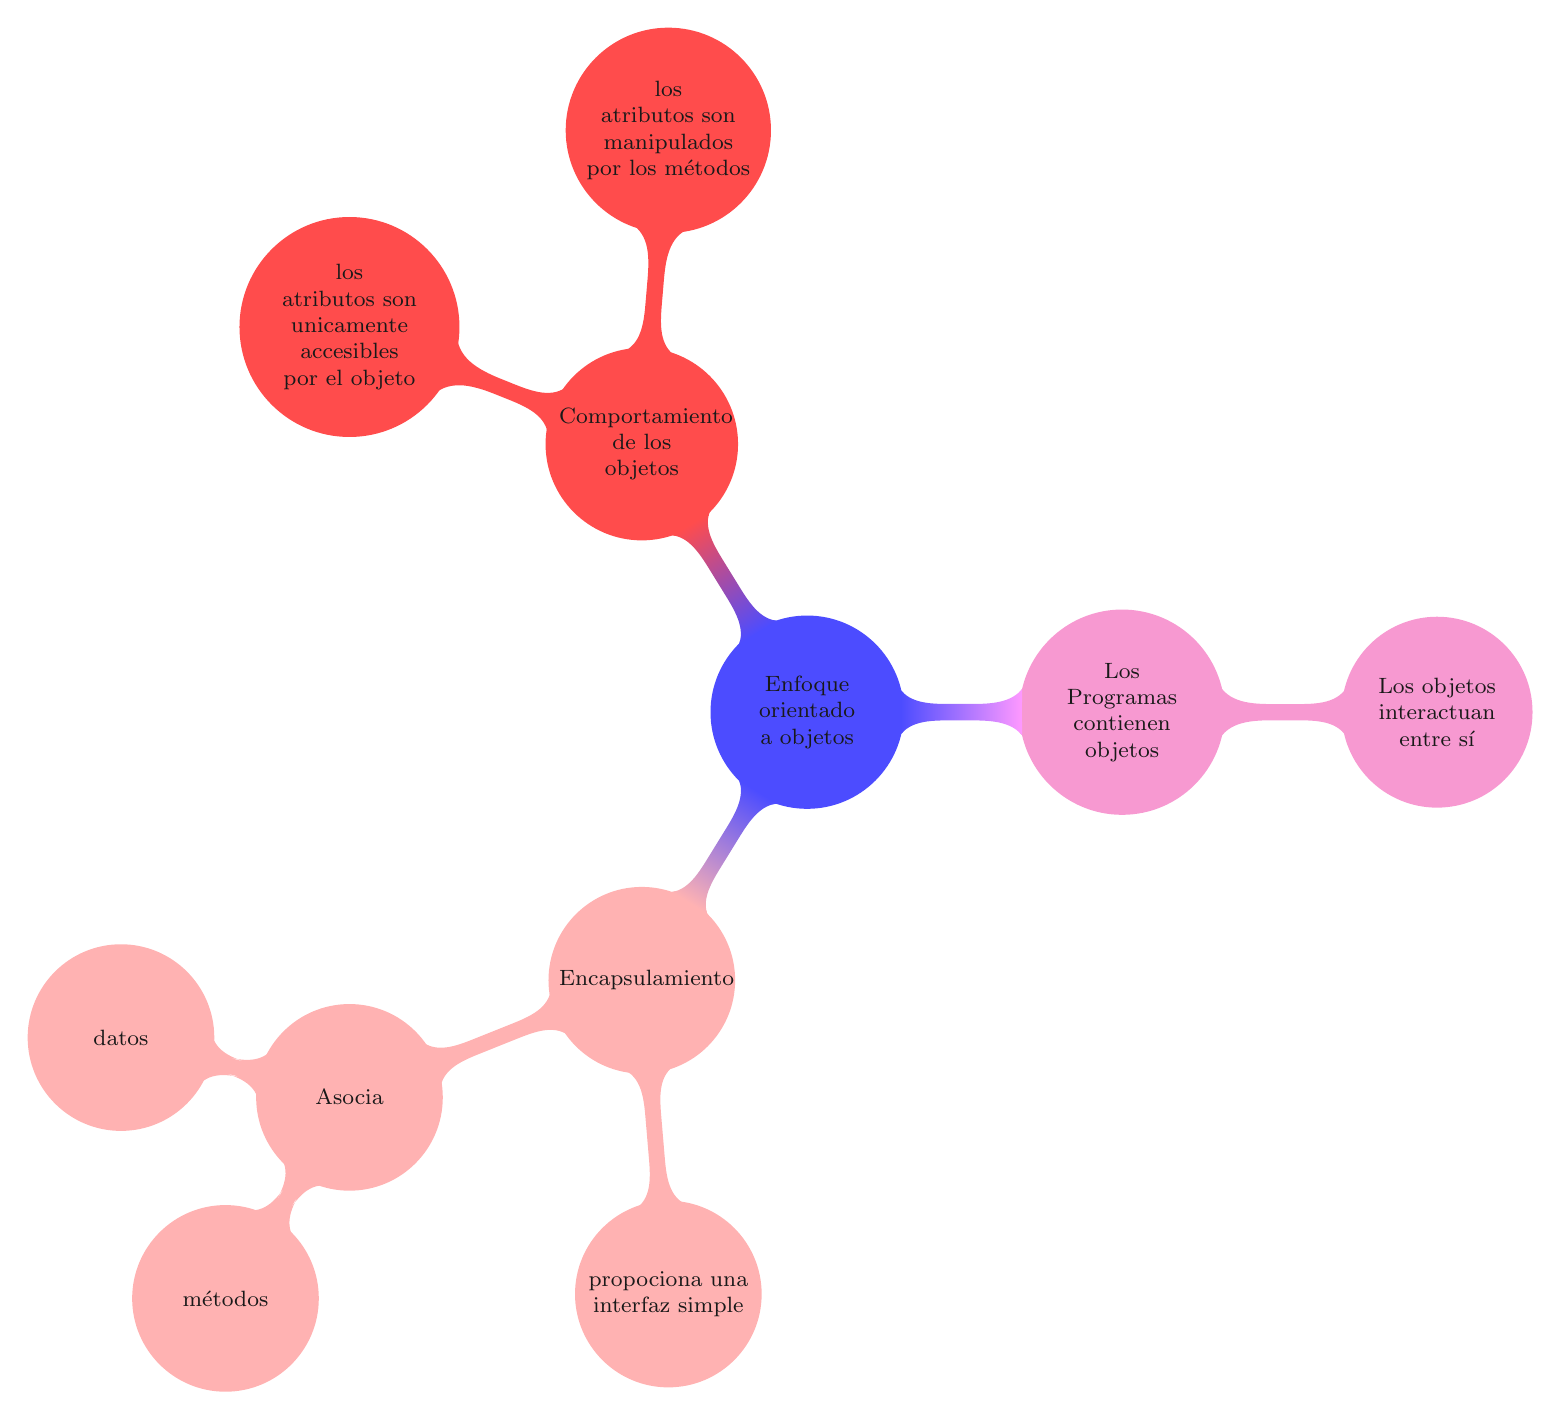
\begin{tikzpicture}[small mindmap, grow cyclic, every node/.style=concept, concept color=blue!70, text=black!90,
        level 1/.style={level distance=4cm, sibling angle=365/3},
        level 2/.style={level distance=4cm, sibling angle=365/5},
        level 3/.style={level distance=3cm, sibling angle=365/5}]
        \node{ Enfoque orientado a objetos }
            child[concept color=pink!120, ] { node { Encapsulamiento }
                child { node { Asocia }
                    child { node { datos } }
                    child { node { métodos } }
                }
            child { node { propociona una interfaz simple } }
            }
            child[concept color=magenta!40] { node { Los\\ Programas contienen objetos }
                child { node { Los objetos interactuan entre sí } }
            }
            child[concept color=red!70] { node { Comportamiento\\ de los\\ objetos }
                child { node { los\\ atributos son\\ manipulados\\ por los métodos } }
                child { node { los\\ atributos son unicamente accesibles por el objeto } }
            }
        ;
\end{tikzpicture}
\end{center}
\end{document}
